% This is samplepaper.tex, a sample chapter demonstrating the
% LLNCS macro package for Springer Computer Science proceedings;
% Version 2.20 of 2017/10/04
%
\documentclass[runningheads]{llncs}
%
\usepackage{graphicx}
\usepackage{amsmath}
\newcommand{\code}[1]{\texttt{#1}}
\usepackage{xcolor}
\usepackage{fancyvrb}
% Used for displaying a sample figure. If possible, figure files should
% be included in EPS format.
%
% If you use the hyperref package, please uncomment the following line
% to display URLs in blue roman font according to Springer's eBook style:
% \renewcommand\UrlFont{\color{blue}\rmfamily}

\begin{document}
%
\title{COMP 472 [or COMP 6721] Template for the Reports \\ (essentially, this is the LNCS template)}
%
%\titlerunning{Abbreviated paper title}
% If the paper title is too long for the running head, you can set
% an abbreviated paper title here
%
\author{First Author\inst{1} \and
Second Author\inst{2} \and
Third Author\inst{3}
\and
Fourth Author\inst{4}}
%
\authorrunning{COMP 472 [or COMP 6721] F. Author et al.}
% First names are abbreviated in the running head.
% If there are more than two authors, 'et al.' is used.
%
\institute{ID-number1 \email{your@email1.com} \and
ID-number2 \email{your@email2.com} \and
ID-number3 \email{your@email3.com} \and
ID-number4 \email{your@email4.com}}
%
\maketitle              % typeset the header of the contribution
%
%
%

\section{Heuristics}

We defined 2 heuristics used by the Best-First Search and A* algorithms. They are as follows: 

\begin{equation}
% h_1(s) = 
% \Bigl\lfloor\dfrac{N^{(s)}_1}{5}\Bigr\rfloor\qquad
h_1(s) = \left\lfloor\dfrac{N^{(s)}_1}{5}\right\rfloor
\end{equation}

\begin{equation}
h_2(s) = N^{(s)}_1
\end{equation}

where $s$ denotes the current state and $N^{(s)}_1$ denotes the number of black dots in state $s$. Both heuristics count the number of black dots to estimate the cost of the cheapest path to the goal state. \\

In $h_1$, we make the simplifying assumption that any move can flip up to 5 arbitrary nodes. Under this assumption, the cheapest path to reach the goal would simply be to flip 5 black dots at each step until all dots are white. This heuristic is intuitive since any move by the player must flip 5 dots, but it fails to discriminate between states whose number of black dots have the same quotient when divided by 5. \\

For example, consider arbitrary states $s_1 =$ \code{111110000} and $s_2 =$ \code{100000000} represented in string form. Then both $h_1(s_1) = 1$ and $h_2(s_2) = 1$, even though $s_2$ is a more desirable state by number of black dots alone. \\

The main strength of $h_1$ is that it is an admissible heuristic. This is true because $h_1$ assumes any move flips $min(5,N^{(s)}_1)$ black dots and 0 white dots, whereas in reality a move would flip \emph{at most} 5 black dots, with the remaining dots flipped being white. In addition, $h_1$ is clearly a consistent heuristic, which makes the A* algorithm optimal under $h_1$ \cite{ref_2} \textcolor{red}{(For peter norvig's book)} \\

$h_2$, on the other hand, simply counts the number of black dots on the board. This heuristic fixes the problem $h_1$ had in discriminating between states that were clearly different. Going back to our example, $h_2(s_1) = 5$ whereas $h_2(s_2) = 1$. \\

However, $h_2$ is not an admissible heuristic, since it over-estimates the cost to reach the goal in at least 1 case, namely when the only 5 black dots on the board are arranged in a cross shape. Here, $h_2(s) = 5$ when the true cost is 1. \\

Both heuristics suffer from the fact that the composition of the board is never taken into account. That is, they both rely solely on the number of black dots to estimate the cost function. On the other hand, both $h_1$ and $h_2$ are extremely simple heuristics to calculate, making them intuitive and their evaluations fast. \\

\section{Difficulties}

\textcolor{red}{(This section might repeat what is said in kabir's section, specifically recursive vs iterative)} \\

Difficulties arose in the first implementation of algorithm A*. We initally decided to implement both algorithms recursively to combat the memory limitations of the iterative DFS. However, we needed a way to keep a running count of the number of nodes visited to date instead of only during the current call stack. \\

Passing in a \code{path\_length} variable to every call to \code{recursive\_a\_star()} and checking whether it hits a limit would only count the depth of a search down a given branch. Therefore, we ended up defining a simple \code{Counter} class that would be passed into every call to \code{recursive\_a\_star()} and count the number of calls. Using the \code{Counter} would avoid the counter resetting at the completion of each recursive call stack. \\

However, we soon realized that such an approach (without a closed list) would make the algorithm unable to distinguish between new and recurrent states, causing loops or repeated visits to certain states. It was ultimately decided that an iterative algorithm would perform much better, since the closed list is only limited by a constant $max_l$, whereas the in the DFS case, the closed list grew exponentially due to the branching factor. \textcolor{red}{(Not sure if matteo's explaining this in his part)}


\section{Analysis and Experiments}

We compare the results and performance of both heuristics for the iterative algorithm on our predefined test cases. \\

For our first test case, both heuristics perform identically, searching the same 4 nodes and reaching the same solution of 2 moves. Furthermore, we know from the properties of $h_1$ that this solution is optimal. \\

For our second case, only $h_2$ manages to find a solution while visiting less than $max_l=100$ nodes. This is likely due to the fact that $h_1$ does not actively try to reduce the number of black dots when searching. This, coupled with the larger number of states a 3x3 board presents (as opposed to the 2x2) meant that the $h_1$ implementation spent much of its time visiting many irrelevant nodes. \\

Our final test case shows this with a grid size of 4x4 as well. $h_1$ fails to find a solution under the maximum number of nodes while $h_2$ is successful. Again, $h_1$ visits too many nodes that don't lead to  a more favorable position. To illustrate this idea further, throughout the search path, $h_2$ never visits a state $s$ with $g(s) > g(s_0)$, where $s_0$ denotes the starting state. $h_1$, on the other hand, unable to discriminate easily between nodes, visits many states with $g(s) = g(s_0)$. (See appendix A)  \\

In order to analyse time and memory usage, we set an unlimited number of nodes to visit in our search. This ensures that we can accurately compare both heuristics by examining their asymptotic performance (i.e., letting the algorithms solve each grid). \\

The results are as follows:

\begin{table}
    \centering
    \caption{A* runtimes and memory usage with $h_1$}\label{tab1}
    \begin{tabular}{|c|c|c|c|}
        \hline
        \textbf{Puzzle size} & \textbf{Max nodes} & \textbf{Runtime} & \textbf{Average memory used} \\
        \hline
        2x2 & $\infty$ & $\sim$ 0.03 seconds & 15.0MiB \\ \hline
        3x3 & $\infty$ & $\sim$ 1.4 seconds & 17.5MiB \\ \hline
        4x4 & $\infty$ & $\sim$ 10.4 seconds & 18.7MiB \\ \hline
    \end{tabular}
\end{table}
\begin{table}
    \centering
    \caption{A* runtimes and memory usage with $h_2$}\label{tab2}
    \begin{tabular}{|c|c|c|c|}
        \hline
        \textbf{Puzzle size} & \textbf{Max nodes} & \textbf{Runtime} & \textbf{Average memory used} \\
        \hline
        2x2 & $\infty$ & $\sim$ 0.06 seconds & 13.5MiB \\ \hline
        3x3 & $\infty$ & $\sim$ 0.6 seconds & 17.2MiB \\ \hline
        4x4 & $\infty$ & $\sim$ 0.6 seconds & 17.3MiB \\ \hline
    \end{tabular}
\end{table}

We can see again that $h_1$ takes significantly more time than $h_2$ to solve more complicated grids, with the memory usage being modest accross all implementations. Again, detailed memory charts can be found in Appendix B.

\textcolor{red}{(Maybe there should be a paragraph comparing all 3 algos?)}

\section{Appendices}
\subsection{Appendix A}

\begin{figure}
\begin{center}
\begin{BVerbatim}
2 0 2 1010010111001010
3 1 2 0010100101001010
3 2 1 0001100001001010
3 2 1 0010000110000010
3 2 1 0010100100000100
3 1 2 0100000111001010
3 2 1 0100000101000110
3 2 1 0100000110000100
3 2 1 0100100100000010
3 1 2 0110110111001010
3 2 1 0110010100000010
...
4 2 2 0110111110111000
4 3 1 0111000010000100
4 2 2 0111000011001010
4 3 1 0111100000000010
4 3 1 1000000000010100
4 3 1 1000000010001011
4 3 1 1000000100000010
4 3 1 1000001000101000
4 2 2 1000001001100110
4 3 1 1000001001000001
4 3 1 1000001010000011
\end{BVerbatim}
\caption{Search path output of A* under $h_1$ on 4x4 test case. The third number represents the value of $g(s)$} \label{fig1}
\end{center}
\end{figure}

\newpage

\begin{figure}
\begin{center}
\begin{BVerbatim}
8 0 8 1010010111001010
7 1 6 0010100101001010
6 2 4 0010000110000010
6 3 3 0001000010000010
6 2 4 0010100100000100
6 3 3 0001100000000100
7 2 5 0001100001001010
7 1 6 0100000111001010
6 2 4 0100000110000100
6 3 3 0100000100001000
6 2 4 0100100100000010
6 3 3 1000000100000010
7 2 5 0100000101000110
7 1 6 1010010110000100
7 2 5 1000001010100100
7 3 4 1000001000101000
7 3 4 1000011001000000
7 2 5 1001010010000100
7 3 4 1001000001100000
7 3 4 1001010000001000
7 2 5 1010000101100000
7 2 5 1010010100001000
7 1 6 1010110100000010
7 2 5 0110010100000010
7 3 4 0100001000100010
7 4 3 0100000001010000
7 3 4 0101010000000010
7 2 5 1000101000100010
7 3 4 1000100001010000
7 2 5 1001110000000010
7 4 3 1100100000000000
5 5 0 0000000000000000
\end{BVerbatim}
\caption{Search path output of A* under $h_2$ on 4x4 test case. The third number represents the value of $g(s)$} \label{fig2}
\end{center}
\end{figure}

\newpage

\subsection{Appendix B}

\begin{figure}
\begin{center}
    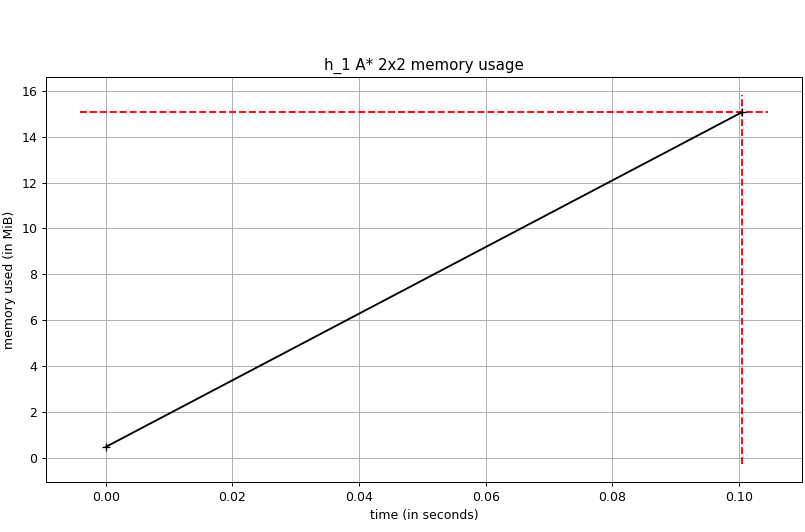
\includegraphics[width=10cm]{a_star_h1_2x2.png}
    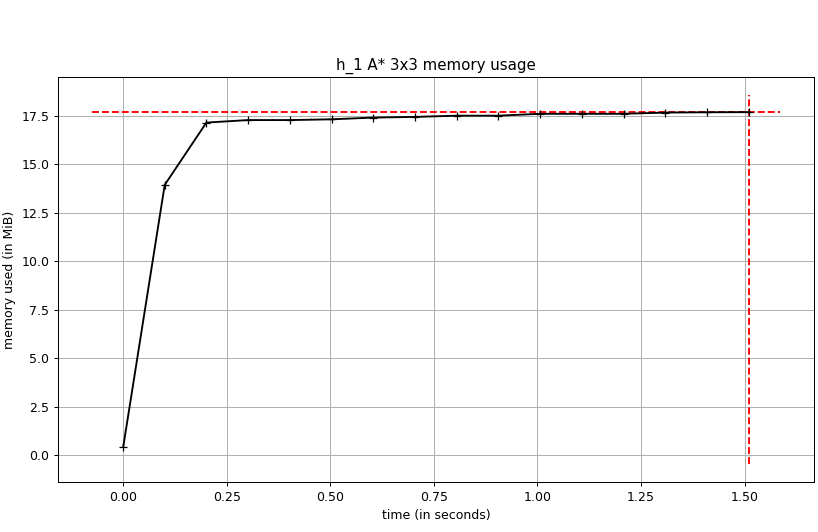
\includegraphics[width=10cm]{a_star_h1_3x3.png}
    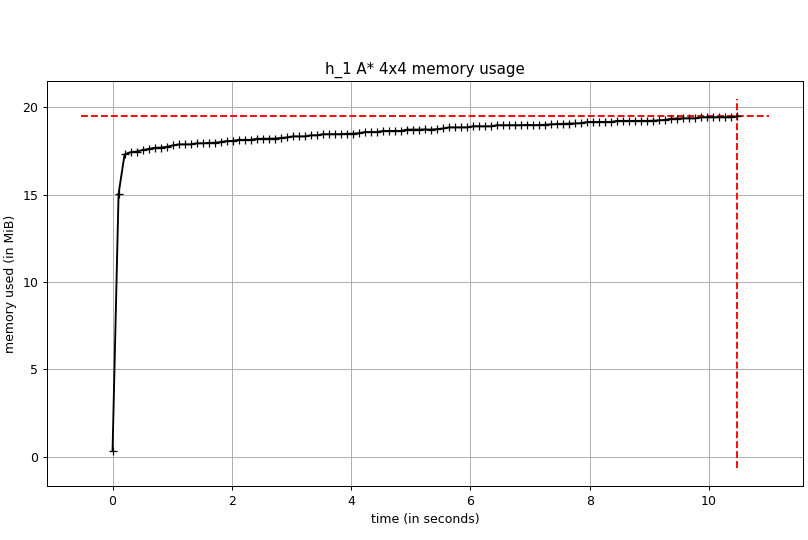
\includegraphics[width=10cm]{a_star_h1_4x4.png}
    \caption{Memory usage of A* under $h_1$} \label{fig3}
\end{center}
\end{figure}

\begin{figure}
\begin{center}
    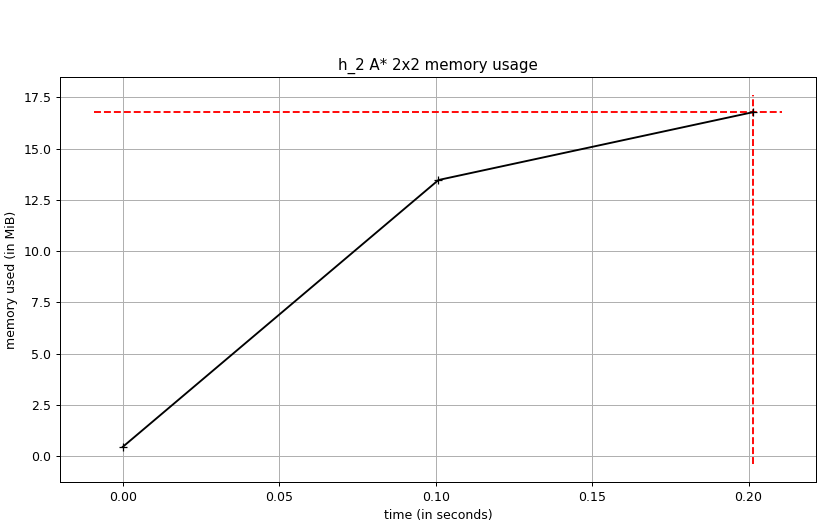
\includegraphics[width=10cm]{a_star_h2_2x2.png}
    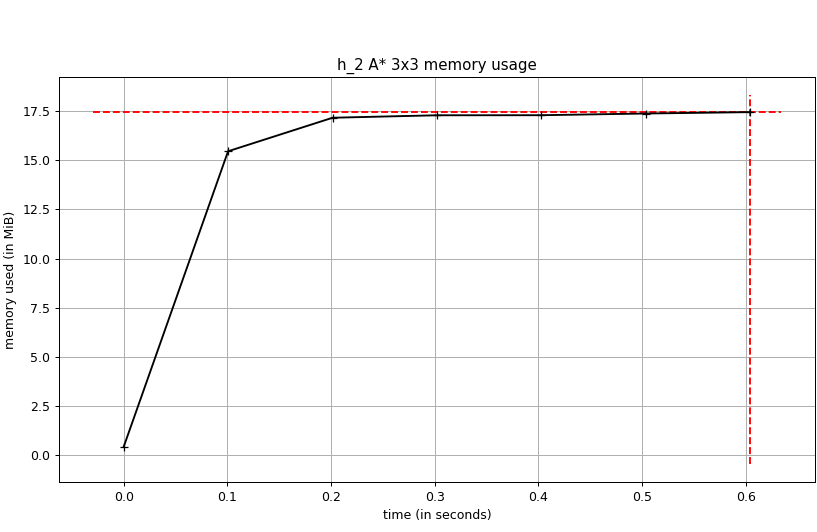
\includegraphics[width=10cm]{a_star_h2_3x3.png}
    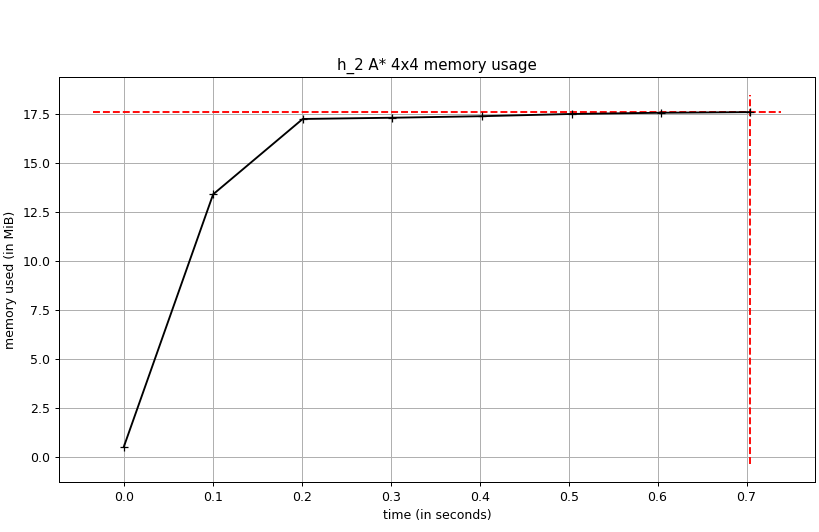
\includegraphics[width=10cm]{a_star_h2_4x4.png}
    \caption{Memory usage of A* under $h_2$} \label{fig4}
\end{center}
\end{figure}

\end{document}
